% Options for packages loaded elsewhere
\PassOptionsToPackage{unicode}{hyperref}
\PassOptionsToPackage{hyphens}{url}
%
\documentclass[
  twoside]{article}
\usepackage{amsmath,amssymb}
\usepackage{iftex}
\ifPDFTeX
  \usepackage[T1]{fontenc}
  \usepackage[utf8]{inputenc}
  \usepackage{textcomp} % provide euro and other symbols
\else % if luatex or xetex
  \usepackage{unicode-math} % this also loads fontspec
  \defaultfontfeatures{Scale=MatchLowercase}
  \defaultfontfeatures[\rmfamily]{Ligatures=TeX,Scale=1}
\fi
\usepackage{lmodern}
\ifPDFTeX\else
  % xetex/luatex font selection
\fi
% Use upquote if available, for straight quotes in verbatim environments
\IfFileExists{upquote.sty}{\usepackage{upquote}}{}
\IfFileExists{microtype.sty}{% use microtype if available
  \usepackage[]{microtype}
  \UseMicrotypeSet[protrusion]{basicmath} % disable protrusion for tt fonts
}{}
\makeatletter
\@ifundefined{KOMAClassName}{% if non-KOMA class
  \IfFileExists{parskip.sty}{%
    \usepackage{parskip}
  }{% else
    \setlength{\parindent}{0pt}
    \setlength{\parskip}{6pt plus 2pt minus 1pt}}
}{% if KOMA class
  \KOMAoptions{parskip=half}}
\makeatother
\usepackage{xcolor}
\usepackage[left=0.75in, right=0.75in, top=0.8in,
bottom=0.4in]{geometry}
\usepackage{graphicx}
\makeatletter
\def\maxwidth{\ifdim\Gin@nat@width>\linewidth\linewidth\else\Gin@nat@width\fi}
\def\maxheight{\ifdim\Gin@nat@height>\textheight\textheight\else\Gin@nat@height\fi}
\makeatother
% Scale images if necessary, so that they will not overflow the page
% margins by default, and it is still possible to overwrite the defaults
% using explicit options in \includegraphics[width, height, ...]{}
\setkeys{Gin}{width=\maxwidth,height=\maxheight,keepaspectratio}
% Set default figure placement to htbp
\makeatletter
\def\fps@figure{htbp}
\makeatother
\setlength{\emergencystretch}{3em} % prevent overfull lines
\providecommand{\tightlist}{%
  \setlength{\itemsep}{0pt}\setlength{\parskip}{0pt}}
\setcounter{secnumdepth}{-\maxdimen} % remove section numbering
\usepackage[charter]{mathdesign}
\usepackage{fancyhdr}
\pagestyle{fancy}
\lhead{CS/MA-135, Hunter, Spring 2024}
\rhead{Name: \hspace{2in}}
\cfoot{}
\setlength{\headsep}{0.2in}

\usepackage{enumitem}
\usepackage{xhfill}

\setenumerate{leftmargin=*}

\ifLuaTeX
  \usepackage{selnolig}  % disable illegal ligatures
\fi
\IfFileExists{bookmark.sty}{\usepackage{bookmark}}{\usepackage{hyperref}}
\IfFileExists{xurl.sty}{\usepackage{xurl}}{} % add URL line breaks if available
\urlstyle{same}
\hypersetup{
  hidelinks,
  pdfcreator={LaTeX via pandoc}}

\author{}
\date{\vspace{-2.5em}}

\begin{document}

\hypertarget{prework-1.3a-regular-expressions}{%
\subsection{Prework 1.3a: Regular
Expressions}\label{prework-1.3a-regular-expressions}}

Write your preliminary solutions to each problem on this sheet of paper
(front and back). The names in brackets indicate the subset responsible
for presenting the problem.

\begin{enumerate}
\def\labelenumi{\arabic{enumi}.}
\item
  {[}Ben, Grace{]} Give a regular expression that describes the language
  consisting of all strings in \(\Sigma = \{a,b\}\) that have an even
  number of a's and an odd number of b's but do not contain the
  substring ab.
\item
  {[}Joshua, Allie{]} Consider the language described by the regular
  expression \(a(abb)^*\cup b\). Use the construction of the proof of
  Lemma 1.55 to build an NFA that recognizes this language.
\item
  {[}Micah, Todd, Curtis{]} Consider the language described by the
  regular expression \((0\cup 1)^*000(0\cup 1)^*\). Use the construction
  of the proof of Lemma 1.55 to build an NFA that recognizes this
  language.
\item
  {[}Andrew, Meghan, David{]} A \emph{generalized nondeterministic
  finite automaton} (GNFA) is a version of an NFA where the edges can be
  labeled with regular expressions, not just symbols. A GNFA accepts a
  string if the parts of the string match the regular expressions as you
  move along the arrows. Consider the GNFA below, and the strings
  \texttt{aa}, \texttt{aababaabbb}, \texttt{aaabab}. Which of these
  strings does it accept?
\end{enumerate}

\begin{center}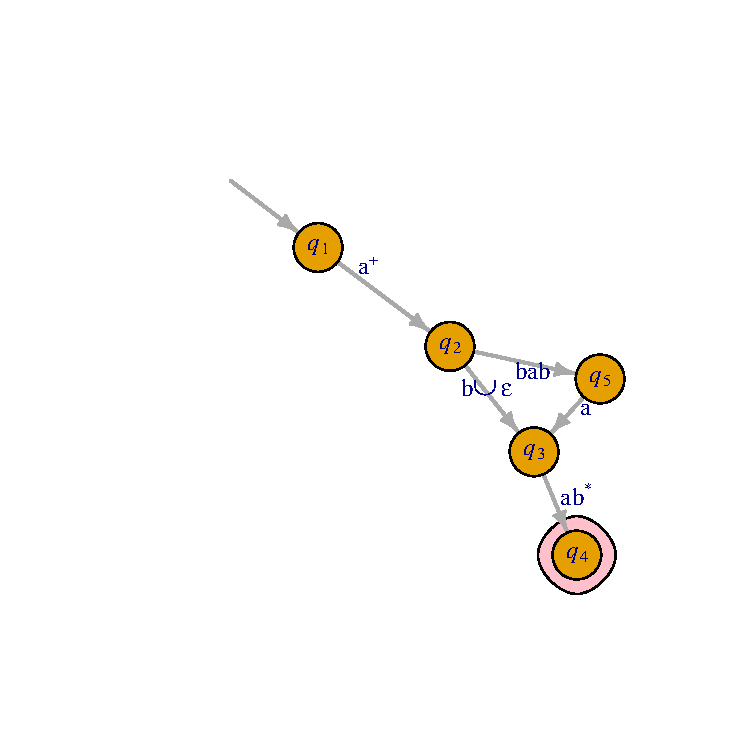
\includegraphics{p13Areg_exp_files/figure-latex/unnamed-chunk-2-1} \end{center}

\begin{enumerate}
\def\labelenumi{\arabic{enumi}.}
\setcounter{enumi}{4}
\tightlist
\item
  {[}Ky, Connor, Levi{]} Modify the GNFA in Problem 4 to create a new
  GNFA with only four states that recognizes the same language. Do this
  by deleting state \(q_5\) and modifying the label on the arrow from
  states \(q_2\) to \(q_3\).
\end{enumerate}

\medskip

\mbox{}\xrfill[2pt]{1pt}\textsc{\small begin your solutions below this line}\xrfill[2pt]{1pt}\mbox{}

\end{document}
